\documentclass[a4paper, twocolumn, final]{ncr_abstract}


% ----------------------------------------------------------------------------
% NCR abstract template file, to be used with ncr_abstract.cls 
%
% Read author instructions on the NCR website carefully before submission of 
% LaTeX based abstracts.
%
% Contact: secretary@ncr-web.org or koen.berends@deltares.nl
% ----------------------------------------------------------------------------

% ----------------------------------------------------------------------------
% For review purposes, you may use line numbers. to show line numbers, uncomment
% below strings and add the \linenumbers command after the frontmatter
% Disable line numebers before submission!!!

%\usepackage{lineno}
%\modulolinenumbers[1]

% Only use the provided bibliography style (do not edit lines below)
\bibliographystyle{model2-names}\biboptions{authoryear}
% ----------------------------------------------------------------------------

\begin{document}
	

	\begin{frontmatter}
		% The title of your abstract
		% ---------------------------------------------------------------------
		\title{Modelling dune evolution under a discharge wave}
	    \specialpapernotice{\hspace{1cm}}
		
		% If you are an invited speaker (e.g. Keynote), uncomment below line
		%\specialpapernotice{\normalsize(\textit{Invited Paper})}	

		% Authors and affilitations
		% ---------------------------------------------------------------------
		\author[UT]{Jord J. Warmink\corref{mycorrespondingauthor}}
		\cortext[mycorrespondingauthor]{Corresponding author}
		\ead{j.j.warmink@utwente.nl}
		\ead[url]{www.utwente.nl}
		
		
		\address[UT]{University of Twente, Department of Water Engineering and Management, Faculty of Engineering Technology, P.O. Box 217, 7500 AE, Enschede, the Netherlands}
		
		% Keywords
		% ---------------------------------------------------------------------
		\begin{keyword}
			River Dunes \sep Time-lag
		\end{keyword}
		
	\end{frontmatter}
	
	% Abstract content
	% ---------------------------------------------------------------------
	% Note: NCR abstracts do not use numbered sections. Always use the 
	% asterisk for headings, as shown below.

	\section*{Introduction}
	Accurate forecasts of flood levels are essential for flood management. During floods, bed forms develop on the river bed. Dunes have heights in the order of 10-30\% of the water depth and lengths in the order of 10 times their height. River bed forms act as roughness to the flow, thereby significantly influencing the (flood) water levels. It is essential to predict the time evolution of bed forms and assess their influence on the hydraulic roughness.

	Field observations have shown that dunes of different lengths and amplitude co-exist (e.g. \cite{Wilbers2003}). \cite{Carling2000} distinguished three scales of bed forms, ripples, small dunes (length \textless 5 m) and large dunes (length \textgreater 10 m) in the German river Rhine and show that the latter two strongly interact.
	
	Several successful attempts were made to model bed form evolution and associated roughness using detailed numerical modeling (e.g. \cite{Nabi2010}). However, these models require long computational times and are therefore not applicable for operational flood management. \cite{Paarlberg2010} developed a process-based model for bed form evolution that requires limited computational effort. This model accounts for flow separation and is able to predict bed form development towards equilibrium conditions. However, the interaction with secondary bed forms is currently not included in the model. Therefore, the objective of this research is to explain and model the interaction between primary and secondary bed forms during a discharge wave measured in a flume.

	\subsection*{Observations from data}
	We compared the flume data from \cite{Wijbenga1986} who imposed two discharge waves in the flume, with the field data from \cite{Wilbers2003} of two discharge waves of 1995 and 1998 in the river Rhine and Waal in the Netherlands. This showed that dune height evolution is similar in the flume and in the field, but the decrease of dune length in the flume is not visible in the field measurements, where dune length only seems to grow. To explain the observed decrease in bed form length in the flume and field data, we propose an hypothesis based on super-imposition of secondary bed forms (\ref{fig:evolution}). The key is that dune length of an individual dune never decreases, but only increases and that secondary bed forms are responsible for the observed decrease in bed form length, because they develop on top, and during decreasing discharge, they become dominant. Because these secondary dunes have a smaller length, the dune length rapidly decreases.
	\begin{figure*}[!b]
	\centering
		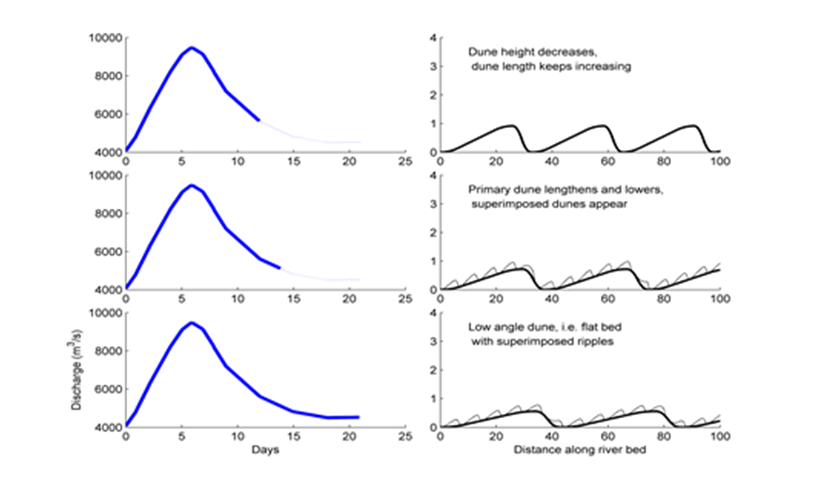
\includegraphics[width=0.6\textwidth]{example_figures/evolution.PNG}
		\caption{Proposed model of bed form evolution during the receding limb of the flood wave. Left: discharge wave of 1995 in Rhine. Right: illustration of dune development (height and length observed in the Rhine in 1995 from \cite{Wilbers2003}}
		\label{fig:evolution}
	\end{figure*}

	\section*{Time-lag approach}
	We applied a time-lag approach for the flume data. \cite{Coleman2005} adopted the commons scaling relationship for sand-wave development from an initially flat bed:
	\begin{equation}
		\frac{P}{P_e} = (\frac{t}{t_e})^\gamma
	\end{equation}
	\noindent where $P$ is the average value of dune length or height, $P_e$ is the equilibrium value, $t$ is time, $t_e$ is the time to achieve $P_e$, and $\gamma$ is a growth rate parameter. \cite{Coleman2005} derived a relation for $\gamma$, based on flume experiment with a discharge step. They showed that growth rate was different for dune height and length and mainly depended on sediment size. Using this approach for the data from \cite{Wijbenga1986} yielded $\gamma_H=0.42$ and $\gamma_H=0.37$.
	\cite{Coleman2005} used their data to derive the te for dunes:
	\begin{equation}
	t_e\left[\frac{u_\ast}{D_{50}}\right] = 2.05\cdot 10^{-2}\left[\frac{D_{50}}{h}^{-3.5}\right]\left[\frac{\theta}{\theta_{cr}}^{-1.12}\right]
	\end{equation}
	They assumed that the times to equilibrium are equal for dune height and dune length, based on flume experiments with a sudden step in discharge that show that after a certain period of time dunes reach their equilibrium. However, observed dune heights during a flood wave from \cite{Wijbenga1986} show that the maximum dune height is reached long before the maximum dune length is reached (Fig. 2). Calibration showed that for dune height, the te values need to adapted with a factor 0.01 to yield realistic dune heights for the \cite{Wijbenga1986} data.
	\begin{figure}
		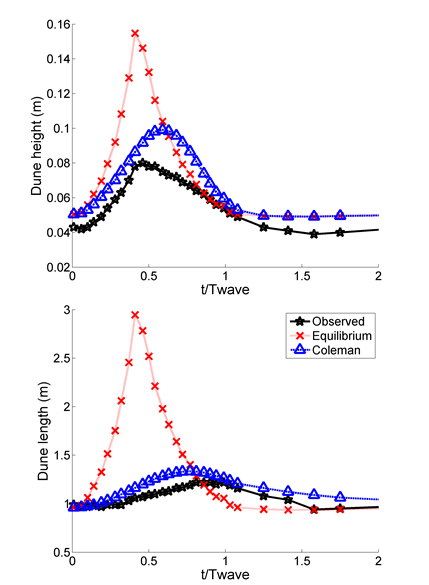
\includegraphics[width=\columnwidth]{example_figures/prediction.PNG}
		\caption{Dune height and dune length prediction using the time-lag approach. The crosses show the $P_e$ predictions}
		\label{fig:prediction}
	\end{figure}

	Fig. \ref{fig:prediction} shows the predicted dune height and length using this time-lag approach. The times to equilibrium, $t_e$, ranged between 3 to 320 days. These values seem unrealistic, but resulted in a reasonably good fit to the observed dune dimensions. Calibration of te for dune height only was required by multiplying te by 0.01. This is not feasible and limits the practical applicability for flood forecasting. Furthermore, the process of overtaking of the primary dunes by the secondary dunes is not taken into account.

	
	% Acknowledgements
	% ---------------------------------------------------------------------
	% Note: You are not required to acknowledge NCR. This is an example
	{\small
		\section*{Future work \& Acknowledgements}
		Further research will focus on validation of the proposed hypothesis and including this process in Paarlberg model for flood forecasting. This study is carried out as part of the project ‘BedFormFlood’, supported by the Technology Foundation STW, the applied science division of NWO and the technology programme of the Ministry of Economic Affairs. 
	}
		
	% references section
	% ---------------------------------------------------------------------
	\section*{References}

	% If you use bibtex to generate your referenc, manually copy the contents of the 
	% resultant *.bbl file here. Do  not submit the .bbl file. 
	\begin{thebibliography}{1}
		\small
		% Article
		\bibitem[{Carling et~al.(2000)}]{Carling2000}
		\bibinfo{author}{Carling, P.A.}, \bibinfo{author}{G\"olz, E.},
		\bibinfo{author}{Orr, H.G.}, \bibinfo{author}{Radecki-Pawlik, A.}, \bibinfo{year}{2000}.
		\newblock \bibinfo{title}{The morphodynamics of fluvial sand dunes in the River Rhine near Mainz, Germany. I. Sedimentology and morphology}.
		\newblock \bibinfo{journal}{Sedimentology}
		  \bibinfo{volume}{47}, \bibinfo{pages}{227--252}.
		% Article
		\bibitem[{Coleman et~al.(2005)}]{Coleman2005}
		\bibinfo{author}{Coleman, S.E.},
		\bibinfo{author}{Zhang, M.H.},
		\bibinfo{author}{Clunie, T.M.},
		\bibinfo{year}{2005}.
		\newblock 
		\bibinfo{title}{Sediment-wave development in subcritical water flow}.
		\newblock 
		\bibinfo{journal}{J. Hydr. Eng.}
		\bibinfo{volume}{131}, \bibinfo{pages}{106--111}.
		% Article
		\bibitem[{Nabi (2010)}]{Nabi2010}
		\bibinfo{year}{2010}.
		\newblock 
		\bibinfo{title}{Computational modelling of three-dimensional bedform evolution}.
		\newblock 
		\bibinfo{journal}{Proc. River Flow 2010}
		\bibinfo{pages}{905-911}.
		% Article
		\bibitem[{Paarlberg et~al.(2010)}]{Paarlberg2010}
		\bibinfo{author}{Paarlberg, A.J.},
		\bibinfo{author}{Dohmen-Janssen, C.M.},
		\bibinfo{author}{Hulscher, S.J.M.H.},
		\bibinfo{author}{Temes, P.},
		\bibinfo{author}{Schielen, R.M.J.},
		\bibinfo{year}{2010}.
		\newblock 
		\bibinfo{title}{Modelling the effect of time-dependent river dune evolution on bed roughness and stage.}.
		\newblock 
		\bibinfo{journal}{Earth Surface Processes and Landforms}
		\bibinfo{volume}{35}, \bibinfo{pages}{1854-1866}.
		% TechReport
		\bibitem[{Wijbenga and Van Nes(1986)}]{Wijbenga1986}
		\bibinfo{author}{Wijbenga, A.},
		\bibinfo{author}{Van Nes, A.R.},
		\bibinfo{year}{1986}.
		\newblock 
		\bibinfo{title}{Flow resistance and bedform dimensions for varying flow conditions; results of flume experiments with flood waves. WL|Delft Hydraulics. Report M1314 part XIII, Delft, the Netherlands.}.
		% Article
		\bibitem[{Wilbers and Ten Brinke(2003)}]{Wilbers2003}
		\bibinfo{author}{Wilbers, A.W.E.},
		\bibinfo{author}{Ten Brinke, W.B.M.},
		\bibinfo{year}{2003}.
		\newblock 
		\bibinfo{title}{The response of subaqueous dunes to floods in sand and gravel bed reaches of the Dutch Rhine}.
		\newblock 
		\bibinfo{journal}{Sedimentology}
		\bibinfo{volume}{50}, \bibinfo{pages}{1013--1034}.

	\end{thebibliography}
	
\end{document}